%%%%%%%%%%%%%%%%%%%%%%%%%%%%%%%%%%%%%%%%%%%%%%%%%%%%%%%%%%%%%%%%%%%%%%%%%%%%%%%%

\section{Analýza}
\label{sec_analyza}

V~této kapitole je analyzován model, který byl popsán v~kapitole~\ref{sec_model}. Sobecký pool disponuje výpočetním výkonem $\alpha$ a zbytek sítě (poctivý těžaři) $1 - \alpha$.

Na obrázku~\ref{fig_markov_chain} je definován potenciální náskok sobeckého poolu jako stochastický proces pomocí Markovova řetězce. Přechody mezi stavy odpovídají vytěžení bloku buďto sobeckým poolem nebo poctivými těžaři. Výskyt těchto událostí odpovídá exponenciálním rozdělení tak, jak bylo popsáno v~sekci~\ref{sec_model_mining_and_pools}. Názvy jednotlivých stavů reprezentují náskok sobeckého poolu. Ten je definován jako rozdíl délek privátní větve sobeckého poolu a veřejné větve blockchainu. Pro shodnou délku obou větví existuje stav $0$ a $0'$. Stav $0$ je stav, ve kterém není blockchain rozvětven. Existuje pouze jeden nejdelší veřejný blockchain a všichni těžaři těží nad stejným blokem.

\begin{figure}[ht]
    \centering
    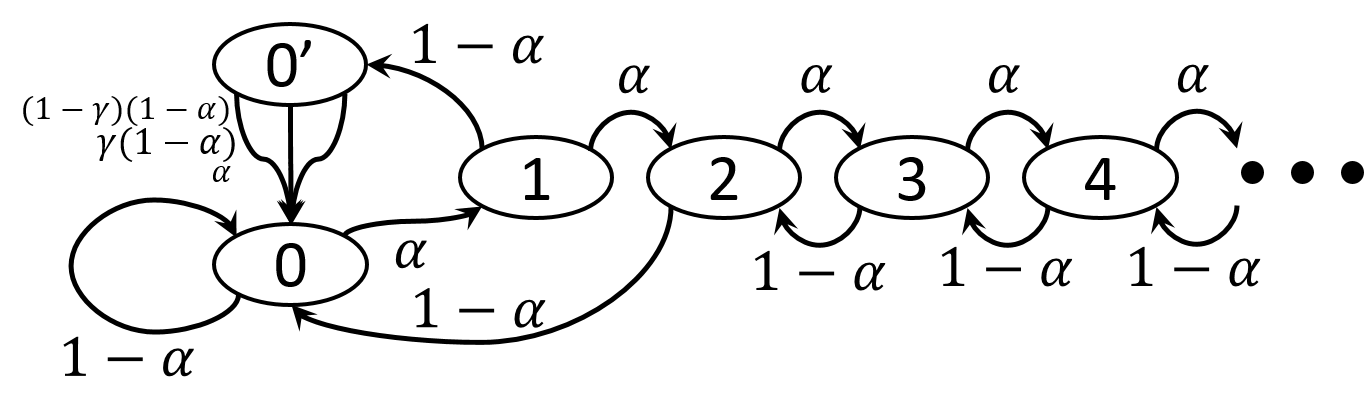
\includegraphics[width=0.8\linewidth]{markov_chain.png}
    \caption{Možný náskok sobeckého poolu popsán jako stochastický proces pomocí Markovova řetězce.}
    \label{fig_markov_chain}
\end{figure}

Stav $0'$ je stav, ve kterém mají obě větve délku od rozvětvení 1. Sobecký pool vytěžil blok první, ale nechal si ho pro sebe. Následně někdo ze zbytku sítě vytežil blok stejné výšky na veřejném blockchainu. Jakmile se sobecký pool o~tomto doví, ihned publikuje svůj dřívě vytěžený blok. Vzniká rozvětvení (\textit{fork}) na veřejném blockchainu. Sobecký pool těží svoji větev. Zbytek sítě podle bitcoinového protokolu těží tu větev, o~které se dozvěděl jako první. Parametrem $\gamma$ definujeme část sítě, která těží větev sobeckého poolu a $1 - \gamma$ část sítě, která těží větev vytěženou někým z~poctivých těžařů. Tento parametr ovlivňuje především latence mezi jednotlivými uzly v~síti.

Pro stavy $s = 0, 1, 2, ...$ platí, že sobecký pool vytěží blok s~pravděpodobností $\alpha$ a tím zvýší svůj náskok na $s + 1$. Ve stavech $s = 3, 4, ...$ platí, že blok vytěží někdo z~upřímných těžařů s~pravděpodobností $1 - \alpha$ a tím sníží náskok sobeckého poolu na $s - 1$. Pokud někdo z~poctivých těžařů vytěží blok ve stavu $s = 2$, sobecký pool zveřejní svoji větev. Jelikož se jedná o~nejdelší blockchain, zbytek sítě opustí svoji práci a dle protokolu přijmou větev sobeckého poolu. Pokud někdo z~poctivých těžařů vytěží blok ve stavu $s = 1$ dostaváme se do již zmíněného stavu $0'$. Z~toho vedou 3 přechody do stavu $s = 0$: (1) sobecký pool vytěží blok nad svoji předchozí privátní větví (pravděpodobnost $\alpha$), (2) někdo z~poctivých těžařů vytěží blok nad větví sobeckého poolu (pravděpodobnost $\gamma \cdot (1 - \alpha)$), (3) někdo z~poctivých těžařů vytěží blok nad veřejnou větví blockchainu (pravděpodobnost $(1 - \gamma) \cdot (1 - \alpha)$).

%%%%%%%%%%%%%%%%%%%%%%%%%%%%%%%%%%%%%%%%%%%%%%%%%%%%%%%%%%%%%%%%%%%%%%%%%%%%%%%%

\subsection{Pravděpodobnost jednotlivých stavů}
\label{sec_analyza_pravdepodobnost}

Nyní spočítejme pravděpodobností rozdělení jednotlivých stavů napříč Markovovým řetězcem. Na základě toho bude možné spočítat očekávané odměny ze sobeckého těžení a porovnat je s~odměnami při standardním chování.

\begin{equation}
    init\_prob\_dist = (P_0, P_{0'}, P_1, P_2, ...) = (1, 0, 0, 0, ...)
    \label{eq_init_prob_dist}
\end{equation}

\begin{equation}
    transition\_matrix =
    \begin{pmatrix}[c|ccccc]
        S_0 & 1 - \alpha & 0 & \alpha & 0 & \cdots \\
        S_{0'} & 1 & 0 & 0 & 0 & \cdots \\
        S_1 & 0 & 1 - \alpha & 0 & \alpha & \cdots \\
        S_2 & 1 - \alpha & 0 & 0 & 0 & \cdots \\
        \vdots & \vdots & \vdots & \vdots & \vdots & \ddots
    \end{pmatrix}
    \label{eq_trans_mat}
\end{equation}

\begin{equation}
    init\_prob\_dist \cdot transition\_matrix^{n} = steady\_state
    \label{eq_steady_state}
\end{equation}

\begin{equation}
    steady\_state \cdot transition\_matrix = steady\_state
    \label{eq_steady_state_2}
\end{equation}

Na rovnici~\ref{eq_init_prob_dist} je definována výchozí rozdělení pravděpodobnosti všech stavů. Na rovnici~\ref{eq_trans_mat} je přechodová matice. Je třeba najít stabilní stav (\textit{steady state} nebo také \textit{stable state}). Ten je definován na rovnici~\ref{eq_steady_state} pro $n \rightarrow \infty$. Pro $steady\_state$ musí platit rovnice~\ref{eq_steady_state_2}. Na základě těchto znalostí, je možné sestavit následující rovnice:

\begin{equation}
    \begin{aligned}
        P_0 &= P_0 \cdot (1 - \alpha) + P_2 \cdot (1 - \alpha) + P_{0'} \\
        P_{0'} &= P_1 \cdot (1 - \alpha) \\
        P_1 &= P_0 \cdot \alpha \\
        \forall k \geq 2 : P_k &= P_{k-1} \cdot \alpha + P_{k + 1} \cdot (1 - \alpha) \\
        0 &= \sum_{i=0}^\infty P_i + P_{0'}
    \end{aligned}
\end{equation}

Vyřešením těchto rovnic získáme \textit{steady state} -- výsledné rozdělení pravděpodobnosti všech stavů. Vyřešení celé soustavy je v~příloze článku~\cite{bib_paper}.

\begin{align}
    \label{eq_probabilities_1}
    P_0 &= \frac{\alpha - 2 \alpha^2}{\alpha \cdot (2 \alpha^3 - 4 \alpha^2 + 1)} \\
    \label{eq_probabilities_2}
    P_{0'} &= \frac{(1 - \alpha) \cdot (\alpha - 2 \alpha^2}{1 - 4 \alpha^2 + 2 \alpha^3} \\
    \label{eq_probabilities_3}
    P_1 &= \frac{\alpha - 2 \alpha^2}{2 \alpha^3 - 4 \alpha^2 + 1} \\
    \label{eq_probabilities_4}
    \forall k~\geq 2 : P_k &= \bigg( \frac{\alpha}{1 - \alpha} \bigg)^{k - 1} \cdot \frac{\alpha - 2 \alpha^2}{2\alpha^3 - 4\alpha^2 + 1}
\end{align}

%%%%%%%%%%%%%%%%%%%%%%%%%%%%%%%%%%%%%%%%%%%%%%%%%%%%%%%%%%%%%%%%%%%%%%%%%%%%%%%%

\subsection{Očekávané odměny}
\label{sec_analyza_odmena}

S~výsledným rozdělením pravděpodobnosti napříč stavovým prostorem již můžeme spočítat očekávané odměny pro sobecký pool a poctivé těžaře. Odměna náleží za vytěžený blok, který je součástí nejdelšího blockchainu. Dále jsou analyzovány odměny pro každý případ, který může nastat.

\begin{enumerate}
    \item[(a)] \textit{Jakýkoliv stav, kromě toho, že délka obou větví je $1$, sobecký pool vytěží blok.} Tím zvyší svůj náskok z~$k$ na $k + 1$. Blok přidá do své privátní větve blockchainu. Odměna bude rozdělena později.

    \begin{figure}[H]
        \centering
        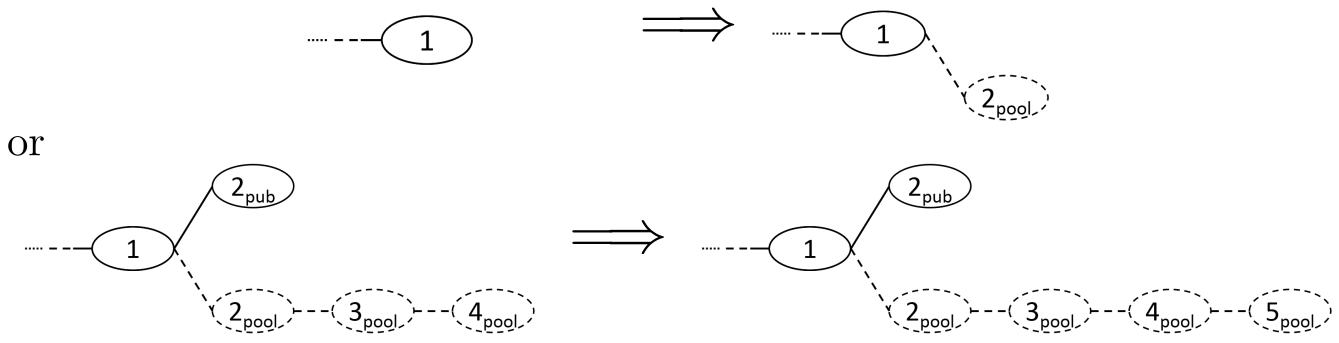
\includegraphics[width=0.99\linewidth]{revenue-case-01.png}
    \end{figure}

    \item[(b)] \textit{Délka obou větví je $1$, sobecký pool vytěží blok.} Tím dosáhne nejdelšího blockchainu, zveřejní svoji větev a získává odměnu za $2$ vytěžené bloky.

    \begin{figure}[H]
        \centering
        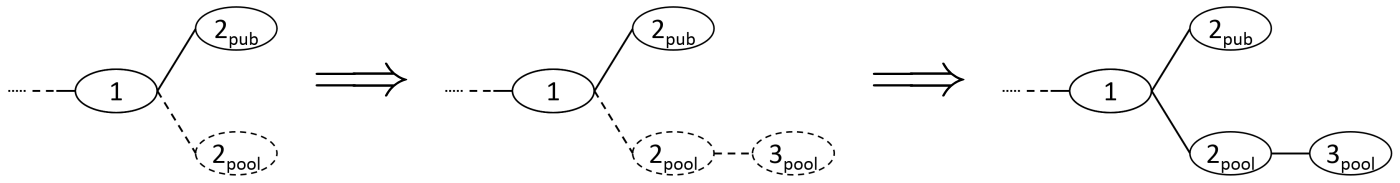
\includegraphics[width=0.99\linewidth]{revenue-case-02.png}
    \end{figure}

    \item[(c)] \textit{Délka obou větví je $1$, ostatní vytěží blok nad blokem sobeckého poolu.} Sobecký pool i zbytek sítě získají každý odměnu za $1$ vytěžený blok -- ostatní za no nově vytěžený blok a sobecký pool za předka.

    \begin{figure}[H]
        \centering
        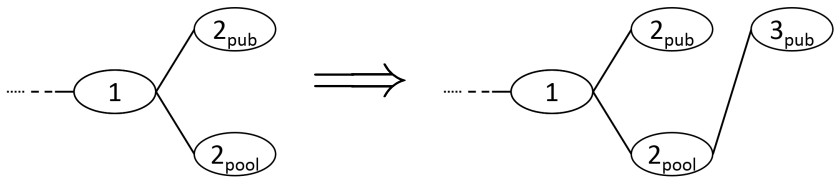
\includegraphics[width=0.7\linewidth]{revenue-case-03.png}
    \end{figure}

    \item[(d)] \textit{Délka obou větví je $1$, ostatní vytěží blok nad blokem ostatních.} Poctiví těžaři získávají odměnu za $2$ vytěžené bloky.

    \begin{figure}[H]
        \centering
        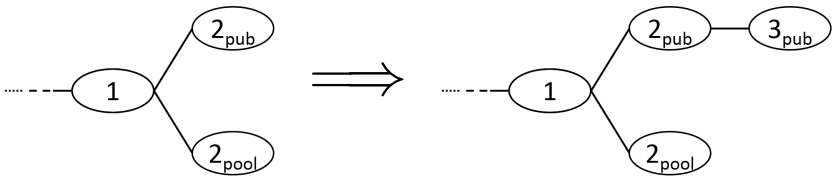
\includegraphics[width=0.7\linewidth]{revenue-case-04.png}
    \end{figure}

    \item[(e)] \textit{Žádná privátní větev neexistuje, všichni v~síti těží nad stejným blokem, upřímní těžaři vytěží blok.} Upřímní těžaři získávají odměnu za 1 vytěžený blok. Všichni začínají těžit nad novým blokem.

    \item[(f)] \textit{Sobecký pool vede o~$1$, ostatní vytěží blok.} Sobecký pool zveřejní svoji větev a vzniká \textit{fork}. Sobecký pool těží nad svoji větví a zbytek sítě se rozdělí podle parametru $\gamma$ -- která verze se k~ním dostane dříve, tu těží. Odměna z~této situace bude rozdělena později, podle toho, která větev "vyhraje".

    \begin{figure}[H]
        \centering
        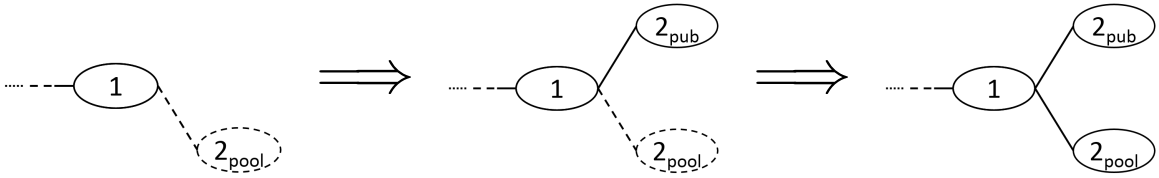
\includegraphics[width=0.9\linewidth]{revenue-case-05.png}
    \end{figure}

    \item[(g)] \textit{Sobecký pool vede o~$2$, ostatní vytěží blok.} Zbytek sítě sníží náskok sobeckého poolu na $1$. Ten jakmile se to dozví, zveřejní celou svoji větev. Jelikož má nejdelší blockchain, všichni přijmou jeho verzi. Sobecký pool obdrží odměnu za $2$ vytěžené bloky.

    \begin{figure}[H]
        \centering
        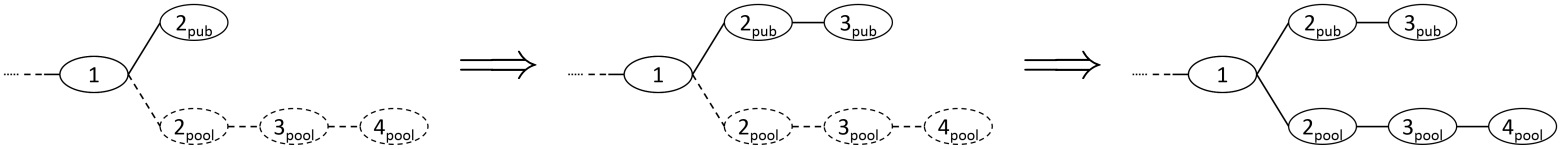
\includegraphics[width=0.99\linewidth]{revenue-case-06.png}
    \end{figure}

    \item[(h)] \textit{Sobecký pool vede o~více než $2$, ostatní vytěží blok výšky $k$.} Zbytek sítě sníží náskok sobeckého poolu, ten zůstává aspoň $2$. Nový blok $k$ od upřímných těžařů nakonec nebude součástí nejdelší blockchainu. Jakmile sobecký pool zveřejní celou svoji větev, ostatní přijmou jeho verzi a on obdrží odměnu za všechny bloky. V~tento okamžik sobecký pool zveřejňuje svůj blok $k$ a získává odměnu za $1$ vytěžený blok.

    \begin{figure}[H]
        \centering
        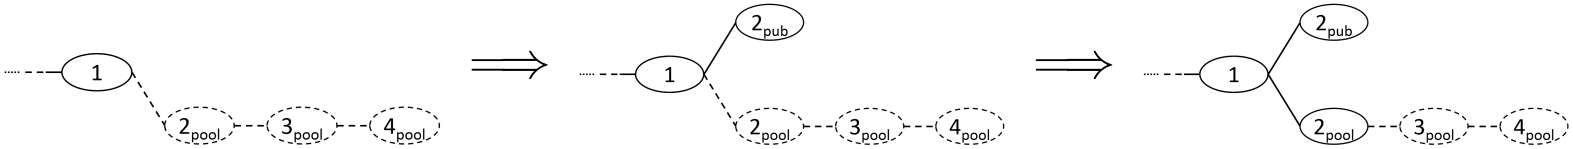
\includegraphics[width=0.99\linewidth]{revenue-case-07.png}
    \end{figure}

\end{enumerate}

Nyní je možné spočítat očekávané odměny sobeckého poolu a poctivých těžařů na základě rozdělení pravděpodobnosti stavů a pravděpodobnosti jednotlivých přechodů.

\begin{equation}
    r_{honest} = \overbrace{1 \cdot P_{0'} \cdot \gamma (1 - \alpha)}^\text{case (c)} +  \overbrace{2 \cdot P_{0'} \cdot (1 - \gamma)(1 - \alpha)}^\text{case (d)} + \overbrace{1 \cdot P_0 \cdot (1 - \alpha)}^\text{case (e)}
    \label{eq_honest_revenue}
\end{equation}

\begin{equation}
    r_{selfish} = \overbrace{2 \cdot P_{0'} \cdot \alpha}^\text{case (b)} + \overbrace{1 \cdot P_{0'} \cdot \gamma (1 - \alpha)}^\text{case (c)} + \overbrace{2 \cdot P_2 \cdot (1 - \alpha)}^\text{case (g)} + \overbrace{1 \cdot P_i \cdot (1 - \alpha)}^\text{case (h)}
    \label{eq_selfish_revenue}
\end{equation}

Podle očekávání záměrné větvení blockchainu sobeckým poolem způsobilo, že poctiví těžaři těžili významnou dobu bloky, které skončily mimo nejdelší blockchain. Toto chování mimo jiné způsobí, že celkové tempo generování nových bloků bude nižší. Obtížnost těžby (nároky na hash bloku) se bude snižovat, aby průměrná doba vytěžení bloku byla $10$ minut.

Dosazením rozdělení pravděpodobnosti stavů z~rovnic~\ref{eq_probabilities_1},~\ref{eq_probabilities_2},~\ref{eq_probabilities_3},~\ref{eq_probabilities_4} do rovnic~\ref{eq_honest_revenue} a~\ref{eq_selfish_revenue} je možné spočítat poměr vytěžených bloků sobeckým poolem ku celkovému počtu vytěžených bloků.

\begin{equation}
    R_{selfish} = \frac{r_{selfish}}{r_{selfish} + r_{honest}} = \cdots = \frac{\alpha (1 - \alpha)^2 (4 \alpha + \gamma (1 - 2 \alpha)) - \alpha^3}{1 - \alpha (1 + (2 - \alpha) \alpha)}
    \label{eq_selfish_revenue_rate}
\end{equation}

%%%%%%%%%%%%%%%%%%%%%%%%%%%%%%%%%%%%%%%%%%%%%%%%%%%%%%%%%%%%%%%%%%%%%%%%%%%%%%%%

\subsection{Simulace}
\label{sec_analyza_simulace}

Pro ověření teoretické analýzy byly výsledky porovnány se simulátorem Bitcoinového protokolu. V~simulaci bylo těžení nahrazeno Monte Carlo simulátorem. Ten simuluje těžení bloků bez skutečného počítání hashů SHA-256 pro různé \textit{nonce}. V~simulaci figurovalo $1000$ těžařů, z~toho $1000 \alpha$ zformovalo sobecký pool. Podrobnější popis simulace je popsán v~článku~\cite{bib_paper} v~sekci 4.3. Obrázek~\ref{fig_simulation} ukazuje, že výsledky simulace odpovídají výsledkům z~teoretické analýzy.

\begin{figure}[H]
    \centering
    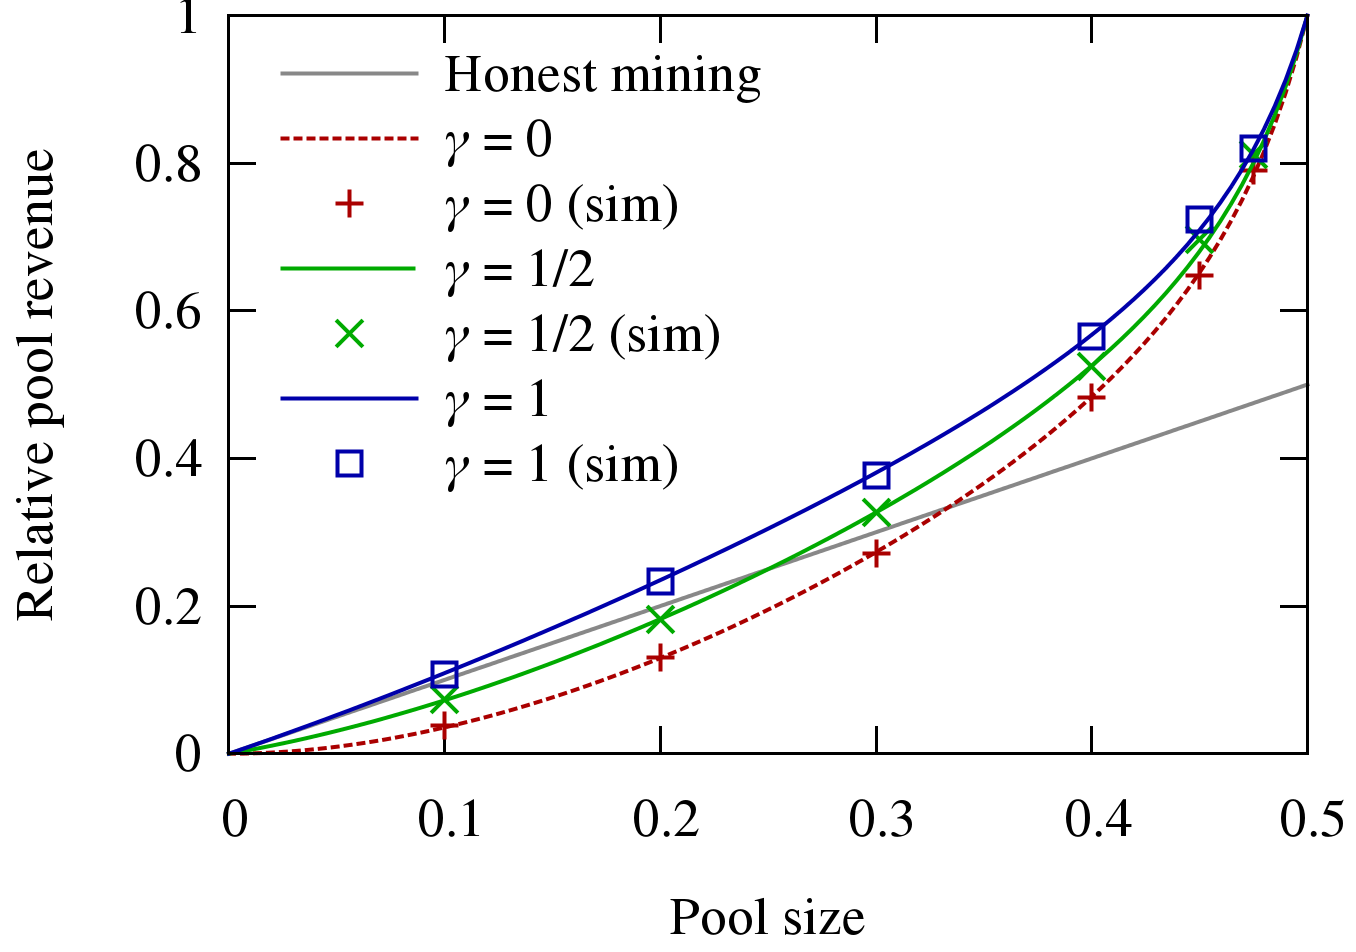
\includegraphics[width=0.68\linewidth]{revenue.png}
    \caption{Odměny ze strategie sobeckého těžení pro různé hodnoty parametru $\gamma$ v~porovnání s~poctivým těžením. Výsledky simulace odpovídají teoretické analýze. A~ukazují, že strategie sobeckého těžení vede od určité hranice k~větším odměnám. Hranice zavisí na parametru $\gamma$.}
    \label{fig_simulation}
\end{figure}

%%%%%%%%%%%%%%%%%%%%%%%%%%%%%%%%%%%%%%%%%%%%%%%%%%%%%%%%%%%%%%%%%%%%%%%%%%%%%%%%

\subsection{Dopady parametrů $\alpha$ a $\gamma$}
\label{sec_analyza_efekt_parametru}

Pokud odměna sobeckého poolu definovaná rovnicí~\ref{eq_selfish_revenue_rate} je vyšší než $\alpha$, tak je strategie sobeckého těžení pro pool výhodnější. Jednotliví těžaři získají vyšší odměnu v~sobeckém poolu než by získali v~poctivých poolech. Nerovnice je platná pouze pro $0 \leq \alpha \leq 0,5$. Nerovnice~\ref{eq_observation_1_p2} je pouze zjednodušení nerovnice~\ref{eq_observation_1_p1}.

\begin{equation}
    \begin{aligned}
        \frac{\alpha (1 - \alpha)^2 (4 \alpha + \gamma (1 - 2 \alpha)) - \alpha^3}{1 - \alpha (1 + (2 - \alpha) \alpha)} > \alpha
    \end{aligned}
    \label{eq_observation_1_p1}
\end{equation}

\begin{theorem}
    Pro konkrétní hodnoty parametru $\gamma$, pool velikosti $\alpha$ získá odměnu větší než náleží jeho relativnímu výpočetnímu výkonu pro $\alpha$ v~rozsahu:

    \begin{equation}
        \begin{aligned}
            \frac{1 - \gamma}{3 - 2 \gamma} < \alpha < \frac{1}{2}
        \end{aligned}
        \label{eq_observation_1_p2}
    \end{equation}
\label{theorem_1}
\end{theorem}

Toto odpovídá výsledkům z~obrázku~\ref{fig_simulation}, kde je zobrazena odměna poolu pro rozdílne hodnoty parametru $\gamma$ pro velikosti poolu od $0$ do $0,5$.

\begin{figure}[ht]
    \centering
    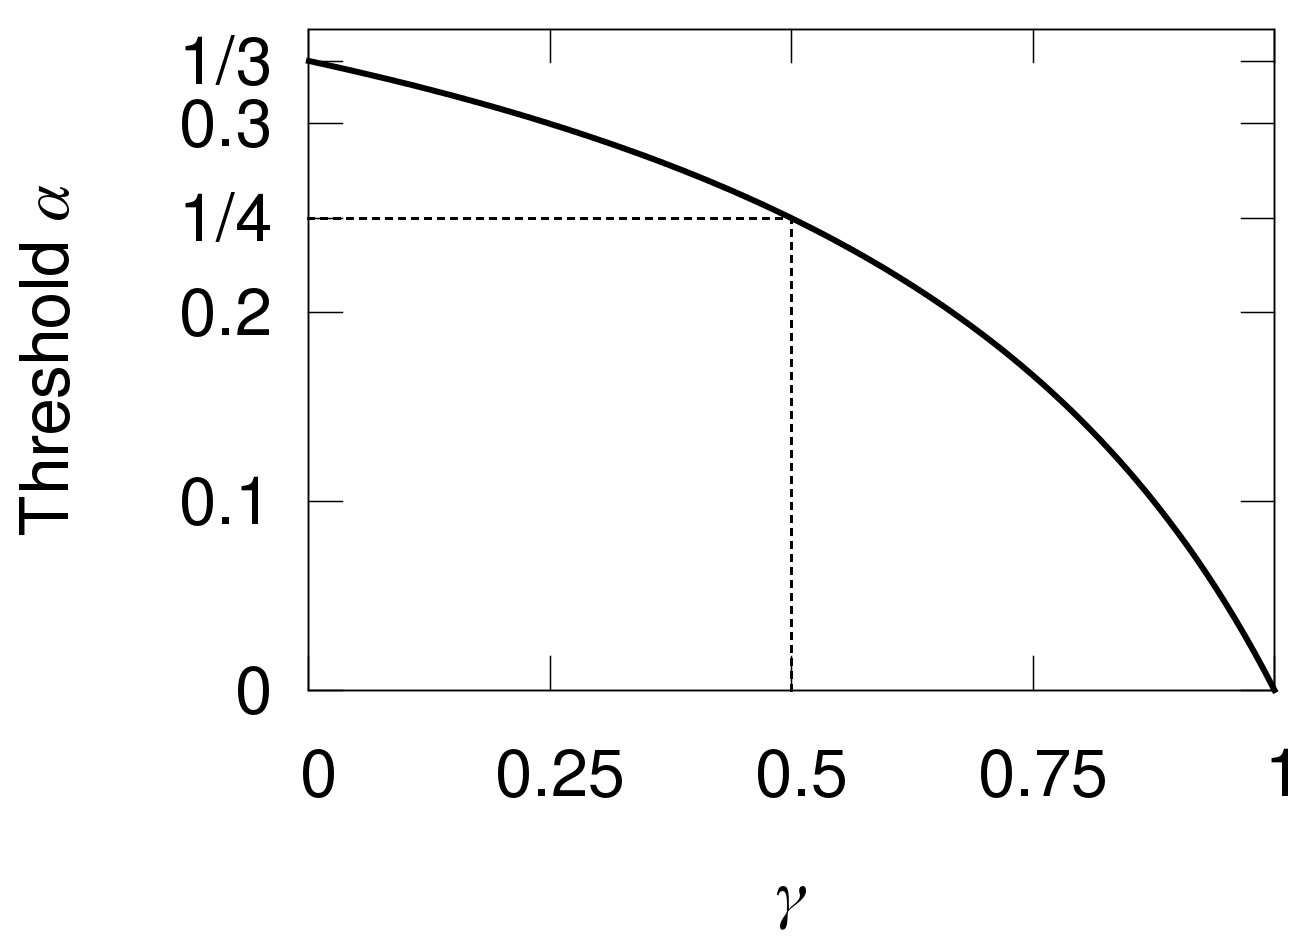
\includegraphics[width=0.5\linewidth]{treshold.png}
    \caption{Hranice pro jaké hodnoty parametrů $\alpha$ a $\gamma$ se vyplatí provozovat strategii sobeckého těžení.}
    \label{fig_treshold}
\end{figure}

Sklon výše odměny poolu $R_{pool}$ jako funkce velikosti poolu je větší než hranice, kdy se vyplatí provozovat strategii sobeckého těžení. Z~toho vyplývá druhý teorém:

\begin{theorem}
    Pro pool provozující strategii sobeckého těžení, se odměna každého člena poolu zvyšuje s~velikostí poolu pro pool větší než je hranice výhodnosti sobeckého těžení nad poctivým těžením.
\label{theorem_2}
\end{theorem}

%%%%%%%%%%%%%%%%%%%%%%%%%%%%%%%%%%%%%%%%%%%%%%%%%%%%%%%%%%%%%%%%%%%%%%%%%%%%%%%%
